% -----------------------------------------------------------------
% 				   Probablility and Statistics
% -----------------------------------------------------------------
\begin{tcolorbox}[colback=cyan!5!white,colframe=cyan!75!black,title=\textbf{Random Variables and Probability}]
\begin{flalign*}
	& \textbf{Dependent Probability: } P(A \lor B) = P(A) + P(B) & \\
	& \textbf{Independent Prob.: } P(A,B) = P(A \land B) = P(A) \cdot P(B) & \\
	& \textbf{Conditional Prob.: } P(A|B) = \frac { P(A|B) }{ P(B) }  =  \frac { P(B|A) \cdot  P(A) }{ P(B) } &
\end{flalign*}
\begin{equation*}
	P(X \in  [a,b]) = \int _{ a }^{ b }{  p_{ X }(x) dx } \hfil p(x|y) = \frac{p(x,y)}{p(y)}
\end{equation*}
\begin{flalign*}
	\textbf{Mean/Expectation value: }
	\mathbb{E} \{\mu_X \} &:= \mu_X = \int_{-\infty}^{\infty}{x \cdot p_X (x) dx } & \\
	\mathbb{E} \{a + bX \} &:= a + b \mathbb{E} \{ X \} &
\end{flalign*}
\begin{flalign*}
	& \textbf{Variance: } \sigma_{X}^{2} := \mathbb{E} \{(X - \mu_X)^2 \} = \mathbb{E} \{ X^2 \} - \mu_{X}^{2} &\\
	& \textbf{Standard deviation: } \sigma_X = \sqrt{\sigma_{X}^{2}} &
\end{flalign*}
\end{tcolorbox}

\begin{tcolorbox}[colback=cyan!5!white,colframe=cyan!75!black,title=\textbf{Distributions}]
\begin{flalign*}
	& \textbf{Uniform distribution:} P_y (x) = \left\{ \begin{matrix} \frac {1}{b-a} & \quad if \quad x  \in  [a,b] \\ 0 & else \end{matrix} \right. & \\
	& \textbf{Mean: } \mu_X = \int_{-\infty}^{\infty}{x \, p_X (x) dx} = \int_{a}^{b}{\frac{1}{b-a} \cdot x dx = \frac{a+b}{2} =: \mu_X} & \\
	& \textbf{Normal distribution: } X \sim \mathcal{N}(\mu, \sigma^2) & \\
	& \hspace{3em}p(x) = \frac{1}{\sqrt{2\pi \sigma^2}}\cdot exp(-\frac{(x-\mu)^2}{2\sigma^2})  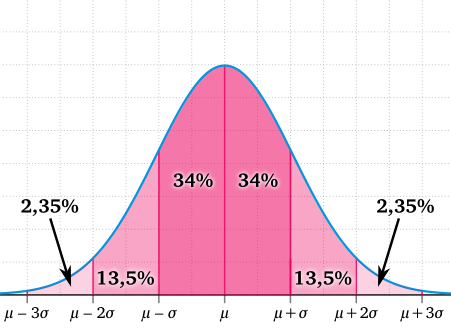
\includegraphics[width = 3cm]{Gauss.png} & \\
	&\textbf{Multidimensional Normal Distribution: } &\\
	& \hspace{1em} p(x)=\frac {1}{\sqrt{(2\pi)^n \cdot det(\Sigma)}} \cdot exp(-\frac{1}{2} \cdot (x-\mu)^T \cdot \Sigma^{-1} \cdot (x-\mu)) & \\
	& \textbf{Weibull distribuation: } F(x) = 1 - e^{-(\lambda \cdot x)^k} & \\
	& \textbf{Laplace distribuation: } f(x|\mu,b) = \frac{1}{2b} \cdot exp \left(-\frac{|x-\mu|}{b}\right) &
\end{flalign*}


%\begin{equation*}
%\text{Variance:} \quad

%\sigma^2 = \frac{ 1 }{ c } \int _{ -\infty  }^{\infty}{y^2 dy} = \frac{ 1 }{ c } \left[ \frac{ 1 }{ 3 } \right]

%\end{equation*}
\end{tcolorbox}

\begin{tcolorbox}[colback=cyan!5!white,colframe=cyan!75!black,title=\textbf{Useful statistic definitions}]
\begin{flalign*}
	& \textbf{Covariance and Correlaton: }	\sigma (X,Y) := \mathbb{E} (X-\mu_X)(Y-\mu_Y) & \\
	& \hspace{3em} = \int_{-\infty}^{\infty} \int_{-\infty}^{\infty} (X - \mu_X)(y - \mu_Y)\cdot p_{X,Y} (x,y)\,  dx \, dy  & \\
	& \textbf{Covariance Matrix: } \Sigma_x = cov(X) = \mathbb{E}\{XX^T\} - \mu_x \mu^T_x  \; \text{is PSD}&
\end{flalign*}
$ \Sigma = \begin{bmatrix}
\sigma_x^2 & \sigma_{yx} \\
\sigma_{xy} & \sigma_y^2
\end{bmatrix}$ \quad $\sigma_{xy} = \sigma{yx} = \rho_{xy} \cdot \sigma_x \cdot \sigma_y$ where $\rho$ is correlation
\textbf{Multidimensional Random Variables:}
\begin{align*}
	\mathbb{E}{f(X)} &= \int_{\mathbb{R}^n}{f(x)p_X(x) d^n x} \\
	cov(X) &= \mathbb{E} \{(X-\mu_X)(X-\mu_X)^T\} \\
	cov(X) &= \mathbb{E} \{XX^T\} - \mu_X \mu_X^T \\
	cov(Y) &= \Sigma_y = A \Sigma_x A^T \quad for \quad y = A \cdot x \\
	\mathbb{E}\{AX\} &=A \cdot \mathbb{ E }\{X\}
\end{align*}
\textbf{Rules for variance: }
\begin{flalign*}
	var(aX) &= {a}^{2} \cdot var(X) &\\
	\hspace{3em} var(X+Y) &= var(X)+var(Y)+2 \cdot cov(X,Y) &
\end{flalign*}
\begin{flalign*}
	 & \textbf{Verschiebesatz: } var(X)= \mathbb{E}((X-\mathbb{E}(X))^2) = \mathbb{E}(X^2)- (\mathbb{E}(X))^2 &
\end{flalign*}
\textbf{Bayes Theorem:}\\
$ P(A\vert B) = \frac{P(A,B)}{P(B)} = \frac{P(B \vert A)P(A)}{P(B)}$\\
\textbf{Correlation:}\\
uncorrelated if $\rho(X,Y) = 0, \; \rho(X,Y) := \frac{cov(X,Y)}{\sigma_x \sigma_y}$
\tcblower

\textbf{Statistical estimators:}
\begin{description}
	\item[\small Biased- and Unbiasedness] An estimator $\hat \theta_N$ is called unbiased iff 	$\mathbb{E}\{ \hat \theta_N (y_N)\} = \theta_0$, where $\theta_0$ is the true value of a parameter. Otherwise, is called biased.
	
	\item[\small Asymptotic Unbiasedness]  An estimator $\hat \theta_N$ is called asymptotically unbiased iff $ \lim\limits_{n \to \infty} \mathbb{E}\{\hat \theta_N (y_N) \} = \theta_0$
	
	\item[\small Consistency] An estimator $\hat \theta_N (y_N)$ is called consistent if, for any $\epsilon > 0$, the probability $P(\hat \theta_N (y_N) \in [\theta_0 - \epsilon, \theta_0 + \epsilon])$ tends to one as $N \rightarrow \infty$.
\end{description}
\end{tcolorbox}

\begin{tcolorbox}[colback=blue!5!white,colframe=blue!75!black,title=\textbf{Unconstrainded Optimization}]
\begin{description}
	\item[\small Theorem 1:](First Order Necessary Conditions)\\
		If $x^* \in D$ is local minimizer of $f : D \rightarrow \mathbb{R}$ and $f \in C^1$ then
		$\nabla f (x^*) = 0$
		Definition (Stationary Point) A point $\bar{x}$ with $\nabla f(\bar{x}) = 0$ is called a stationary point of f.
	
	\item[\small Theorem 2:] (Second Order Necessary Conditions)\\
		If $x^* \in D$ is local minimizer of $f : D \rightarrow R$ and $f \in C^2$ then
		$\nabla^2 f(x^*) \succeq 0$
	
	\item[\small Theorem 3:] (Second Order Sufficient Conditions and Stability under Perturbations)\\
		Assume that $f : D \rightarrow R$ is $C^2.$ If $x^* \in D$ is a stationary point and
		$ \nabla^2 f(x^*) \succ 0$
		then $x^*$ is a strict local minimizer of f. In addition, this minimizer is locally unique and is stable against small perturbations of f, i.e. there exists a constant C such that for sufficiently small $p \in \mathbb{R}^n$ holds\\
		\begin{equation*}
		\lVert{x^* - \underset{x}{arg\,min}  (f(x) + p^T x)}\rVert \leq C \lVert p \rVert
		\end{equation*}	
\end{description}
\end{tcolorbox}